\graphicspath{ {images/employee/} }
\section{Сотрудники}
Раздел \quotes{Сотрудники} содержит в себе различные функции по работе с сотрудниками. 

\subsection{Роли и операции}
Раздел доступен пользователям, имеющим следующие роли:
\begin{itemize}
	\item Администратор Платформы:
	\begin{itemize}
		\item просмотр списка сотрудников;
		\item просмотр подробной информации о сотруднике;
		\item приглашение сотрудника на Платформу;
		\item приглашение сотрудников на Платформу списком;
		\item журнал действий сотрудников;
		\item назначение ролей.
	\end{itemize}
	\item Администратор вуза"=поставщика:
	\begin{itemize}
		\item просмотр списка сотрудников;
		\item просмотр подробной информации о сотруднике;
		\item приглашение сотрудника на Платформу;
		\item приглашение сотрудника на Платформу списком;
		\item просмотр журнала действий сотрудников;
		\item назначение ролей.
	\end{itemize}
\end{itemize}

\subsection{Список сотрудников}
Список сотрудников "--- это табличное представление всех пользователей, 
которым назначены какие"=либо права в рамках данного вуза.
Внешний вид списка представлен на рис.~\ref{img:employee:employee_list}.
Элементы управления табличными представления описаны в подразделе~\ref{sec:datatables}.

\begin{figure}[H]
	\center{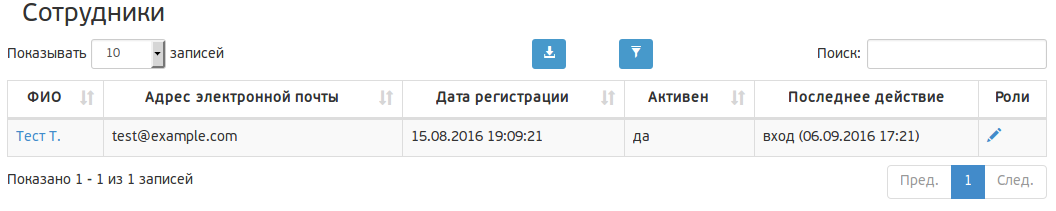
\includegraphics[width=1\linewidth]{employee_list}}
	\caption{Список сотрудников}
	\label{img:employee:employee_list}
\end{figure}


Таблица содержит следующие столбцы:
\begin{itemize}
	\item ФИО сотрудника;
	\item адрес электронной почты;
	\item дата регистрации;
	\item флаг активности;
	\item последнее действие.
\end{itemize}

ФИО сотрудника является ссылкой на просмотр подробной информации о нем, описанной в подразделе~\ref{sec:employee_detail}.
В крайнем правом столбце таблицы находится кнопка перехода к форме редактирования ролей данного сотрудника в рамках данного вуза, 
описание которой находится в подразделе \ref{sec:university_role}.


Внешний вид диалога фильтрации списка сотрудников представлен на рис.~\ref{img:employee:employee_list_filter}.
Можно фильтровать список по следующим полям:

\begin{itemize}
	\item ФИО "--- текстовое поле;
	\item адрес электронной почты "--- текстовое поле;
	\item диапазон дат регистрации "--- виджеты выбора даты и времени 
	(описание виджета см. в подразделе~\ref{widget:date_time_picker});
	\item флаг активности "--- выпадающий список из вариантов да/нет.
\end{itemize}

\begin{figure}[H]
	\center{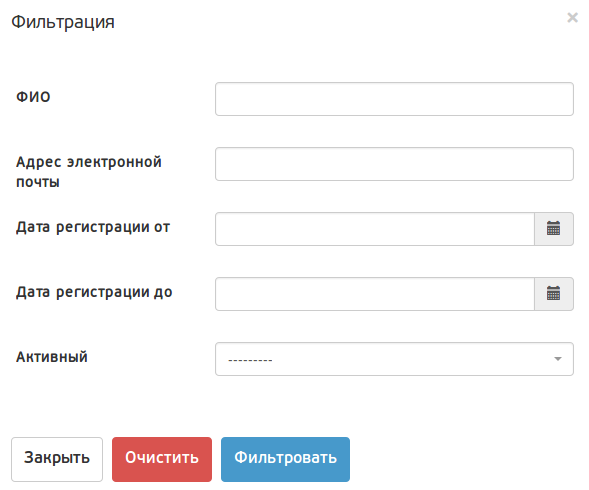
\includegraphics[height=6cm]{employee_list_filter}}
	\caption{Диалог фильтрации списка сотрудников}
	\label{img:employee:employee_list_filter}
\end{figure}


\subsection{Подробная информация о сотруднике} \label{sec:employee_detail}
Внешний вид страницы с подробной информацией о сотруднике представлен на рис.~\ref{img:employee:employee_detail}.
\begin{figure}[H]
	\center{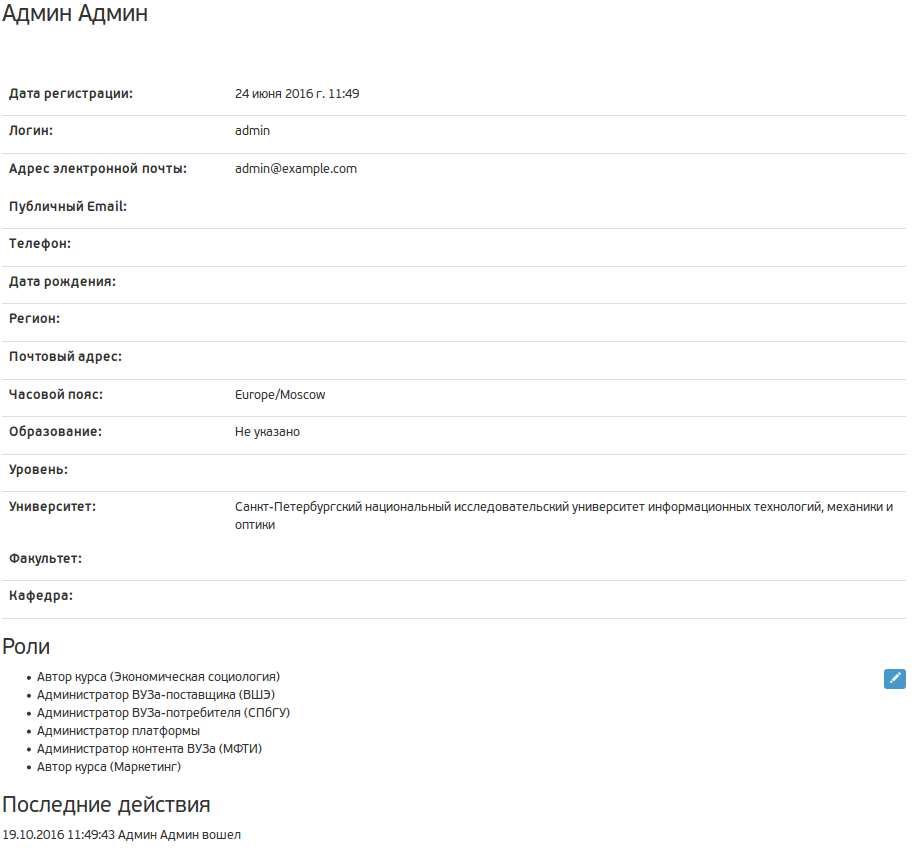
\includegraphics[height=10cm]{employee_detail}}
	\caption{Подробная информация о сотруднике}
	\label{img:employee:employee_detail}
\end{figure}

Для просмотра доступны следующие поля:
\begin{itemize}
	\item дата регистрации;
	\item логин;
	\item адрес электронной почты;
	\item публичный email;
	\item телефон;
	\item дата рождения;
	\item регион;
	\item почтовый адрес;
	\item часовой пояс;
	\item образование;
	\item степень;
	\item университет;
	\item факультет;
	\item кафедра;
	\item список назначенных ролей;
	\item последние действия на Платформе.
\end{itemize}

Рядом со списком ролей пользователя находится кнопка перехода 
к форме редактирования ролей данного сотрудника в рамках данного вуза, 
описание которой находится в подразделе \ref{sec:university_role}.

\subsection{Приглашение сотрудника на Платформу}

Внешний вид формы приглашения сотрудника на Платформу представлен на рис.~\ref{img:employee:invite}. 

\begin{figure}[H]
	\center{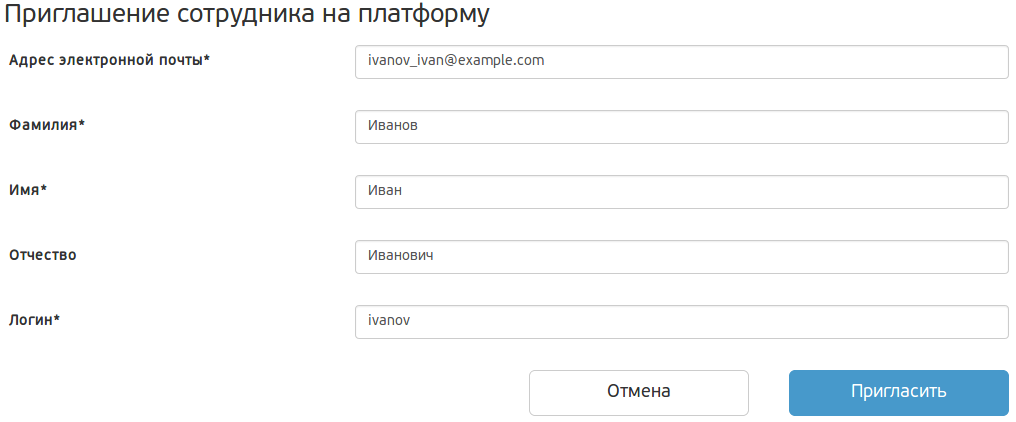
\includegraphics[width=1\linewidth]{invite}}
	\caption{Приглашение сотрудника на Платформу}
	\label{img:employee:invite}
\end{figure}

Для приглашения сотрудника на Платформу необходимо заполнить все поля формы:
\begin{itemize}
	\item адрес электронной почты: ввод информации необходимо осуществлять в корректном формате, например 
	\texttt{npoed@mail.ru}, в противном случае появится сообщение об ошибке и будет заблокирована кнопка сохранения изменений;
	\item фамилия "--- текстовое поле;
	\item имя "--- текстовое поле;
	\item логин "--- текстовое поле.
\end{itemize}

Все поля формы являются обязательными для заполнения, если такое поле оставить не заполненным "--- появляется сообщение 
о необходимости его заполнения и блокируется кнопка сохранения изменений. 
После заполнения всех полей необходимо нажать на кнопку \quotes{Пригласить}.

Так как адрес электронной почты и логин должны быть уникальными для всех пользователей Платформы, в случае указания
уже существующего логина или адреса электронной почты, система выдаст соответствующие ошибки:
\begin{itemize}
	\item пользователь с таким именем пользователя уже зарегистрирован на Платформе;
	\item пользователь с таким e"=mail уже зарегистрирован на Платформе.
\end{itemize}

В случае успеха осуществляется переход на страницу назначения прав приглашенному пользователю в рамках данного вуза 
(см. подраздел \ref{sec:university_role}), а также отображается сообщение \quotes{Приглашение успешно выслано}.

\subsection{Приглашение сотрудников на Платформу списком}
Внешний вид формы приглашения сотрудников на Платформу списком представлен на рис.~\ref{img:employee:mass_invite}. 
Для осуществления приглашения сотрудников списком необходимо нажать на кнопку \quotes{Обзор} и в появившемся диалоге выбрать CSV"=файл 
с заголовками {\tt email}, {\tt last\_name}, {\tt first\_name}, {\tt username} и данными о сотрудниках. 
Шаблон требуемого файла можно скачать, нажав на ссылку \quotes{Скачать шаблон}.

\begin{figure}[H]
	\center{
\includegraphics[width=1\linewidth]{mass_invite}}
	\caption{Приглашение сотрудников списком}
	\label{img:employee:mass_invite}
\end{figure}

После выбора файла необходимо нажать на кнопку \quotes{Загрузить}, после чего начнется загрузка файла и его обработка.
При загрузке некорректного файла могут отобразиться следующие ошибки:
\begin{itemize}
	\item В CSV файле отсутствуют столбцы {\tt email}, {\tt last\_name}, {\tt first\_name}, {\tt username};
	\item CSV файл пустой.
\end{itemize} 

При загрузке корректного файла результаты обработки отображаются в виде двух таблиц: 
первая таблица содержит данные об успешно приглашённых сотрудниках, 
вторая таблица содержит данные о неприглашенных сотрудниках с указанием ошибок. 
Результат приглашения сотрудников представлен на рис.~\ref{img:employee:mass_invite_result}.

\begin{figure}[H]
	\center{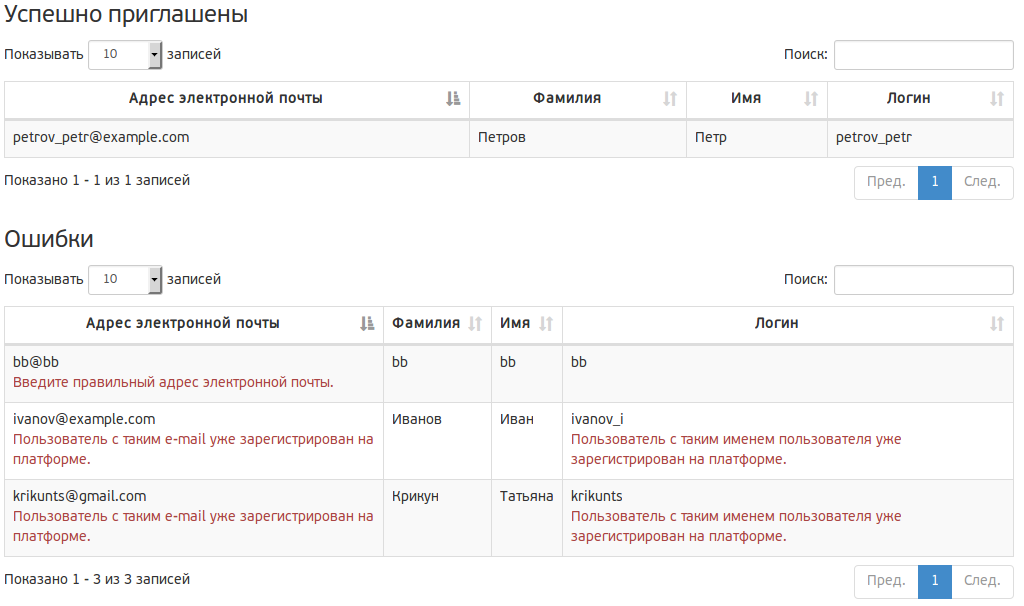
\includegraphics[width=1\linewidth]{mass_invite_result}}
	\caption{Результат приглашения сотрудников списком}
	\label{img:employee:mass_invite_result}
\end{figure}

\subsection{Журнал действий сотрудников}
Журнал действий сотрудников "--- это табличное представление истории действий сотрудников данного вуза на Платформе.
Внешний вид списка представлен на рис.~\ref{img:employee:log_list}. 
Элементы управления табличными представлениями описаны в подразделе~\ref{sec:datatables}.
\begin{figure}[H]
	\center{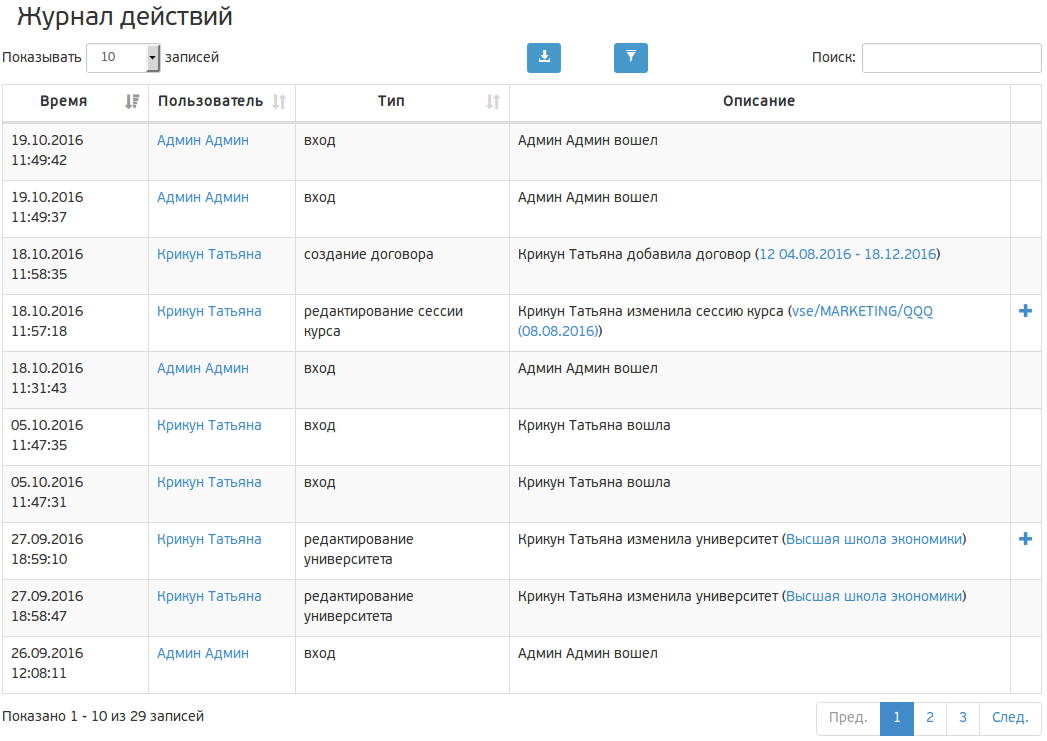
\includegraphics[width=1\linewidth]{log_list}}
	\caption{Журнал действий сотрудников}
	\label{img:employee:log_list}
\end{figure}

Таблица содержит следующие столбцы:
\begin{itemize}
	\item дата и время действия;
	\item сотрудник, совершивший действие;
	\item тип действия;
	\item текстовое описание действия.
\end{itemize}

ФИО сотрудника является ссылкой на просмотр подробной информации о нем, описанной в подразделе~\ref{sec:employee_detail}.

Внешний вид диалога фильтрации журнала действий представлен на рис.~\ref{img:employee:log_list_filter}.
Можно фильтровать список по следующим полям:

\begin{itemize}
	\item диапазон дат действия "--- виджеты выбора даты и времени 
	(описание виджета см. в подразделе~\ref{widget:date_time_picker});
	\item пользователь, совершивший действие "--- виджет выпадающего списка с автодополнением с возможностью множественного выбора 
	(описание виджета см. в подразделе~\ref{widget:autocomplete_with_multiselect});
	\item тип действия "--- виджет выпадающего списка с автодополнением с возможностью множественного выбора
	(описание виджета см. в подразделе~\ref{widget:autocomplete_with_multiselect}).
\end{itemize}

\begin{figure}[H]
	\center{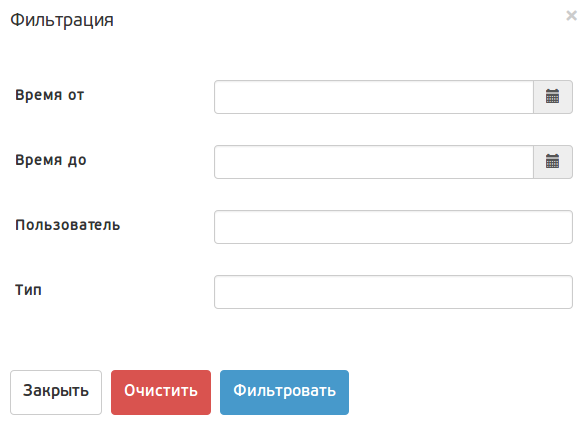
\includegraphics[height=6cm]{log_list_filter}}
	\caption{Диалог фильтрации журнала действий}
	\label{img:employee:log_list_filter}
\end{figure}

В настоящий момент в журнал записываются следующие типы действий:

\begin{itemize}
	\item вход на Платформу;
    \item приглашение на Платформу;
    \item выдача полномочий;
    \item создание университета;
    \item редактирование университета;
    \item создание преподавателя;
    \item редактирование преподавателя;
    \item создание курса;
    \item редактирование курса;
    \item создание сессии курса;
    \item редактирование сессии курса;
    \item зачисление студентов;
    \item отчисление студентов;
    \item изменение режима прохождения курса студентами;
    \item создание заявки на зачисление студентов;
    \item принятие заявки на зачисление студентов;
    \item отклонение заявки на зачисление студентов;
    \item создание заявки на изменение режима прохождения сессии курса студентом;
    \item принятие заявки на изменение режима прохождения сессии курса студентом;
    \item отклонение заявки на изменение режима прохождения сессии курса студентом;
    \item создание договора;
    \item редактирование договора.
\end{itemize}

Некоторые типы событий предполагают наличие в описании события вспомогательных ссылок для упрощения навигации. 
Так, при создании или редактировании университетов, преподавателей, курсов, сессий курсов, 
заявок на зачисление/изменение режима прохождения, договоров между вузом"=разработчиком и вузом"=потребителем,
при принятии или отклонении заявок содержится ссылка на созданную или измененную сущность.


Если тип действия связан с редактированием какой"=либо сущности, то в журнале отображается информация об изменениях, 
внесенных в результате редактирования. Просмотреть подробности изменения можно, 
нажав на кнопку \vcenteredinclude[height=20px]{plus} в крайнем правом столбце таблицы.
Внешний вид внесенных при редактировании изменений представлен на рисунке~\ref{img:employee:log_diff}.
\begin{figure}[H]
	\center{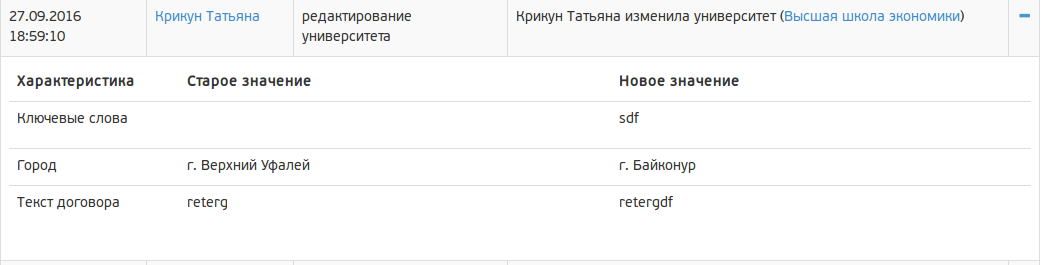
\includegraphics[width=1\linewidth]{log_diff}}
	\caption{Внесенные при редактировании изменения}
	\label{img:employee:log_diff}
\end{figure}

Для каждой измененной характеристики объекта отображается название характеристики, её старое и новое значение.


Для того, чтобы спрятать подробности по данному действию, нужно нажать на кнопку \vcenteredinclude[height=20px]{minus}.

\subsection{Назначение ролей в рамках вуза} \label{sec:university_role}

Назначение ролей в рамках вуза доступно администратору вуза"=поставщика и администратору Платформы. В случае, если у сотрудника
уже есть роли в рамках данного вуза, в форму редактирования прав можно попасть, нажав \vcenteredinclude[height=25px]{edit_btn} в 
таблице с сотрудниками. Если у сотрудника ещё нет ролей в рамках данного вуза, то назначить ему роли можно выбрав пункт 
\quotes{Назначение ролей} в разделе <<Сотрудники>>.

\subsubsection{Назначение ролей из таблицы сотрудников}

При нажатии на кнопку \vcenteredinclude[height=25px]{edit_btn} в таблице сотрудников пользователю будет показана форма, 
аналогичная показанной на рис.~\ref{img:employee:individual_form}. В данной форме будут добавлены уже имеющиеся у пользователя роли
с их параметрами. Все изменения будут сохранены только после нажатия кнопки <<Сохранить>> внизу формы.

\begin{figure}[H]
	\center{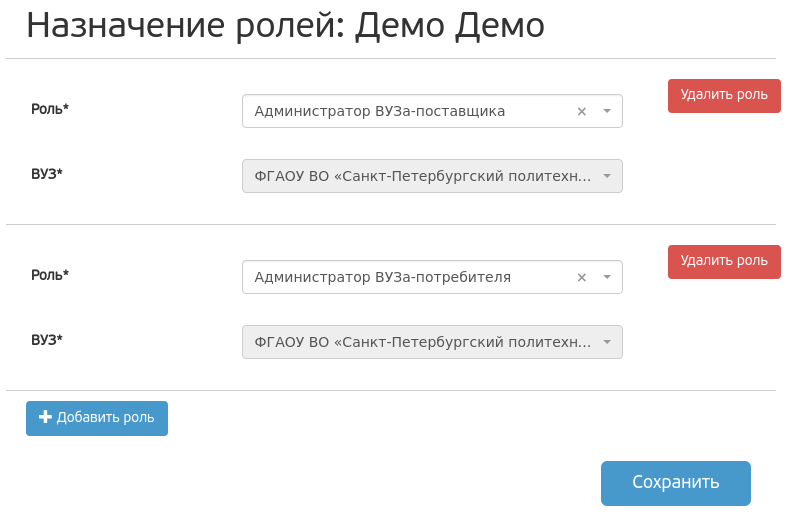
\includegraphics[width=1\linewidth]{individual_form}}
	\caption{Форма назначения ролей для действующего сотрудника}
	\label{img:employee:individual_form}
\end{figure}

Для добавления новой роли необходимо нажать на кнопку <<Добавить роль>> в нижней части формы. В результате появится часть формы для
добавления одной роли, предлагающая выбрать роль для назначения (рис.~\ref{img:employee:choose_role}). В зависимости от 
выбранной роли, на экране появится часть формы для выбора параметра роли. Возможны следующие типы параметров:
\begin{itemize}
	\item {\bf вуз}: неизменяемое поле, в котором выбран текущий вуз (рис.~\ref{img:employee:uni_role});
	\item {\bf курс}: для выбора используется неизменяемое поле <<вуз>> и выпадающий список с автодополнением <<курс>>. 
	Возможен выбор из курсов выбранного университета (рис.~\ref{img:employee:course_role});
	\item {\bf сессия курса}:  для выбора используется неизменяемое поле <<вуз>>, выпадающий список с автодополнением <<курс>>, выпадающий список с автодополнением <<сессия курса>>.  Возможен выбор из сессий выбранного курса, требуется сначала выбрать курс (рис.~\ref{img:employee:session_role}).
\end{itemize}

Описание работы с полями для выбора параметров см. в подразделе~\ref{widget:autocomplete}

\begin{figure}[H]
	\center{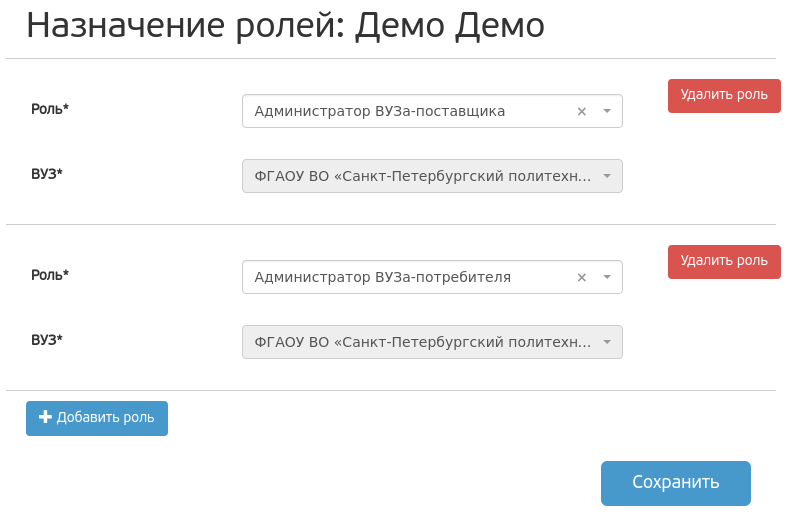
\includegraphics[width=1\linewidth]{individual_form}}
	\caption{Назначение новой роли пользователю: выбор роли}
	\label{img:employee:choose_role}
\end{figure}
\begin{figure}[H]
	\center{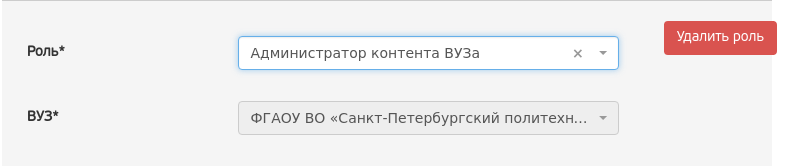
\includegraphics[width=1\linewidth]{uni_role}}
	\caption{Назначение новой роли пользователю: роль с параметром типа <<вуз>>}
	\label{img:employee:uni_role}
\end{figure}
\begin{figure}[H]
	\center{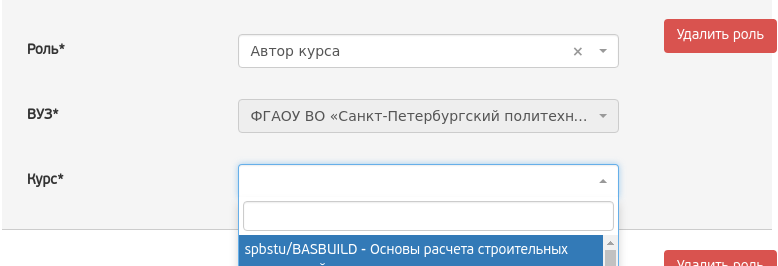
\includegraphics[width=1\linewidth]{course_role}}
	\caption{Назначение новой роли пользователю: Назначение новой роли пользователю: роль с параметром типа <<курс>>}
	\label{img:employee:course_role}
\end{figure}
\begin{figure}[H]
	\center{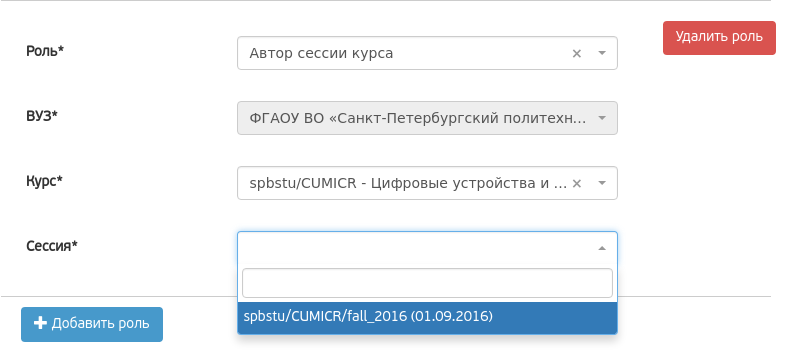
\includegraphics[width=1\linewidth]{session_role}}
	\caption{Назначение новой роли пользователю: Назначение новой роли пользователю: роль с параметром типа <<сессия курса>>}
	\label{img:employee:session_role}
\end{figure}

Для удаления роли нужно нажать кнопку <<Удалить роль>> рядом с выбранной ролью.


\subsubsection{Назначение ролей для новых сотрудников}

При нажатии на пункт \quotes{Назначение ролей} в разделе \quotes{Сотрудники} пользователю показывается форма для выбора пользователя,
которому будут назначаться права (рис.~\ref{img:employee:choose_user_form}). После выбора сотрудника будут загружены имеющиеся роли (если они есть).
Далее работа с формой аналогична работе с формой, описанной в предыдущем разделе.

\begin{figure}[H]
	\center{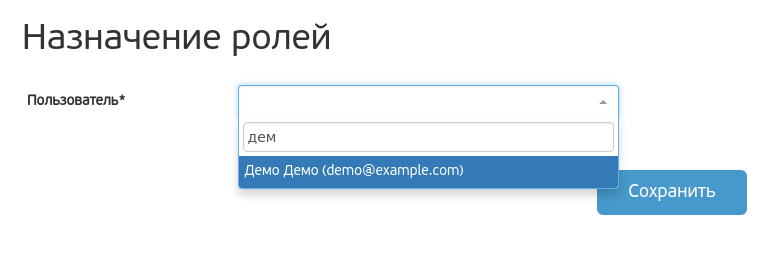
\includegraphics[width=1\linewidth]{choose_user_form}}
	\caption{Форма назначения ролей для нового сотрудника}
	\label{img:employee:choose_user_form}
\end{figure}

\subsection{Назначение глобальных ролей} \label{sec:global_role}

Для администратора Платформы доступна глобальная форма для назначения ролей. Попасть в эту форму можно нажав на пункт <<Назначение ролей>> в
меню <<Мой профиль>> (рис.~\ref{img:employee:global_perms_menu}). Работа с данной формой аналогична работе с формой, описанной в 
подразделе~\ref{sec:university_role}, с некоторыми отличиями:
\begin{itemize}
	\item если для выбора параметра требуется выбор вуза, поле <<вуз>> является выпадающим списком с 
	автодополнением (см. подраздел~\ref{widget:autocomplete});
	\item для выбора доступны роли без параметров (например, <<администратор Платформы>>, рис.~\ref{img:employee:no_param_role});
	\item если для выбора параметра требуется выбор курса, то сначала должен быть выбран вуз"=разработчик курса.
\end{itemize}

\begin{figure}[H]
	\center{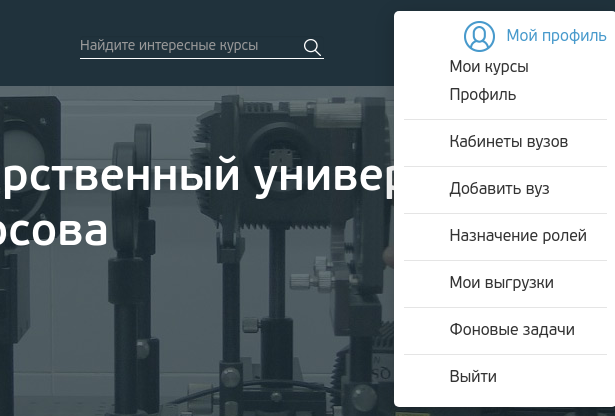
\includegraphics[width=1\linewidth]{global_perms_menu}}
	\caption{Переход на глобальную форму назначения ролей}
	\label{img:employee:global_perms_menu}
\end{figure}

\begin{figure}[H]
	\center{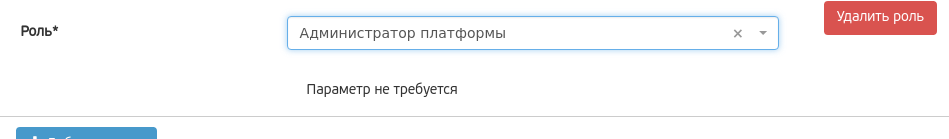
\includegraphics[width=1\linewidth]{no_param_role}}
	\caption{Роль без параметра}
	\label{img:employee:no_param_role}
\end{figure}
